% arara: pdflatex
% !arara: indent: {overwrite: on}
\documentclass{beamer}

\usetheme{CambridgeUS}

%-chage foot part-------------------------------
\makeatother
\setbeamertemplate{footline}
{
  \leavevmode%
  \hbox{%
  \begin{beamercolorbox}[wd=.17\paperwidth,ht=2.25ex,dp=1ex,center]{author in head/foot}%
    \usebeamerfont{author in head/foot}\insertshortauthor
  \end{beamercolorbox}%
  \begin{beamercolorbox}[wd=.46\paperwidth,ht=2.25ex,dp=1ex,center]{title in head/foot}%
    \usebeamerfont{title in head/foot}\insertshorttitle
  \end{beamercolorbox}%
  \begin{beamercolorbox}[wd=.37\paperwidth,ht=2.25ex,dp=1ex,center]{date in head/foot}% 
  \insertdate \hspace{0.2cm}
    \insertframenumber{} / \inserttotalframenumber\hspace*{1ex}
  \end{beamercolorbox}}%
  \vskip0pt%
}
\makeatletter
\setbeamertemplate{navigation symbols}{}
%--------------------------------

%-chage titlepage's font-------------------------------
\setbeamercolor{title}{bg=red!65!black,fg=white}
\usepackage{bm}
\usepackage{comment}
\usepackage{graphics} % used for scalebox
\usepackage{multirow}%used for multicolumn
\usepackage{array}%used for vrule
\usepackage{subfigure}
\usepackage{threeparttable} % used for footnotes in table

%---set tikz highlighter------------------------
\usepackage{multirow, booktabs, dcolumn, color} % Tables
\usepackage[beamer,customcolors]{hf-tikz}
\usetikzlibrary{calc}
% To set the hypothesis highlighting boxes red.
\tikzset{hl/.style={
    set fill color=red!80!black!40,
    set border color=red!80!black,
  },
}
%-----------------------------------------------

%---set tikz marker-----------------------------
\usepackage{tikz}
\usetikzlibrary{positioning}
\tikzset{>=stealth}

\newcommand{\tikzmark}[3][]{\tikz[overlay,remember picture,baseline] \node [anchor=base,#1](#2) {#3};}
%-----------------------------------------------

%---set textblock----------------------------
\usepackage[absolute,overlay]{textpos}
%--------------------------------------------------------

%use bold arrow
\usepackage{marvosym}

\setbeamertemplate{sidebar right}
{
  \vfill%
  \llap{\insertlogo\hskip0.1cm}%
  \vskip2pt%
  %\llap{\href{http://tex.stackexchange.com/}{A link to tex.sx}\hskip0.2cm}% NEW
  \vskip3pt% NEW
  \llap{\usebeamertemplate***{navigation symbols}\hskip0.1cm}%
  \vskip2pt%
}

\begin{document}

\title[Category-Level Transfer Learning from Knowledge Base to Microblog Stream for Accurate Event Detection]{Category-Level Transfer Learning from Knowledge Base to Microblog Stream for Accurate Event Detection}
\author[Weijing Huang, et,al.]{Weijing Huang, Tengjiao Wang, Wei Chen, Yazhou Wang}
\institute[EECS, Peking University]{School of Electronics Engineering and Computer Science, Peking University}
\date{\(\bm{@}\)DASFAA 2017, Suzhou, China}
\maketitle

%------------------------------
%page 2
\begin{frame}
\frametitle{Motivation}

Many Web applications need the \textbf{accurate event detection} technique on microblog stream, including:
\begin{enumerate}
	\item public opinion analysis [Chen, SIGIR 2013]
	\item public security [Li, ICDE 2012], [Imran, WWW 2014]
	\item disaster response [Sakaki,WWW2010]
	\item breaking news report\footnote{\url{http://www.theverge.com/2016/12/1/13804542/reuters-algorithm-breaking-news-twitter}}
\end{enumerate}	
\vfill

But detecting events on twitter stream accurately is still challenging.
\end{frame}

%------------------------------
%page 3
\begin{frame}
\frametitle{Challenges (1/2)}
According to [Huang, WWW 2016], the challenges include,
\begin{enumerate}
\item fast changing
\item high noise
\item short length
\end{enumerate}	

\vfill

And, we found another key factor, 
\begin{enumerate}
\item Small events with fewer tweets \MVRightarrow \ \ Hard to trade off between precision and recall. 
\end{enumerate}




\end{frame}

%------------------------------
%page 4
\begin{frame}
\frametitle{Challenges (2/2)}	
Exploratory study on the \textit{Edinburgh twitter corpus}: 11/29 events contain less than 50 tweets.

\intextsep=5pt plus 3pt minus 1pt % 调整表格与正文的上间距
\begin{table}[]
\setlength{\abovecaptionskip}{0.cm}%set the distance between caption and table to 0 cm.
\setlength{\belowcaptionskip}{0.cm}
\centering
\caption{Statistics of labeled events.}
\label{my-label}
\scalebox{0.65}{
\begin{tabular}{|l|l|r|}
\hline
Event                                        & Date       & Event Size \\ \hline
S\&P downgrade US credit rating                  & 05/08/2011 & 656      \\ \hline
Atlantis shuttle lands                           & 21/07/2011 & 595      \\ \hline
US increases debt ceiling                        & 25/07/2011 & 485      \\ \hline
Plane with Russian hocky team Lokomotiv crashes  & 07/09/2011 & 286      \\ \hline
Amy Winehouse dies                               & 23/07/2011 & 283      \\ \hline
Gunman opens fire in youth camp in Norway        & 23/07/2011 & 260      \\ \hline
Earthquake in Virginia                           & 24/08/2011 & 246      \\ \hline
First victim of London riots dies                & 09/08/2011 & 174      \\ \hline
Explosion in French nuclear plant in Marcoule    & 12/09/2011 & 135      \\ \hline
Google announces plans to bury Motorola Mobility & 15/08/2011 & 127      \\ \hline
NASA announces there might be water on Mars      & 04/08/2011 & 124      \\ \hline
Car bomb explodes in Oslo, Norway                & 22/07/2011 & 114      \\ \hline
... & ... & ... \\ \hline
\tikzmarkin<1>[hl]{bH1}Indian and Bangladesh sign a border pact         & 06/09/2011 & 25       \\ \hline
Flight 4896 crash                                & 13/07/2011 & 21       \\ \hline
First aritficial organ transplant                & 12/07/2011 & 18       \\ \hline
three men die in riots in england                & 10/08/2011 & 16       \\ \hline
rebels capture interational tripoli airport      & 21/08/2011 & 13       \tikzmarkend{bH1} \\ \hline
\end{tabular}
}
\end{table}

 \begin{textblock}{0.1}(13.5,11.7)
  \footnotesize{11 Small events with fewer tweets}
 \end{textblock}

\end{frame}

%\begin{comment}
%------------------------------
%page 5
\begin{frame}
\frametitle{How about existing methods? (1/2)}
Event detection methods \textit{without extra information}, such as
\begin{enumerate}
\item clustering articles
\begin{itemize}
	\item LSH[Petrovic, NAACL 2010]
	\item need to set threshold to determine whether new article represents a new event.
\end{itemize}
\item analyzing word frequencies
\begin{itemize}
	\item EDCoW[Weng, ICWSM 2011]
	\item treat the word as the basic unit in analysis, without regarding polysemy words (words have different meanings, e.g. ``apple")
\end{itemize}
\item finding bursty topics via topic modeling
\begin{itemize}
	\item TimeUserLDA[Diao, ACL 2012], BurstyBTM[Yan, AAAI 2015]
	\item detects the ``large" events but may ignore the ``small" ones. 
\end{itemize}
\end{enumerate}
\end{frame}

\begin{frame}
\frametitle{How about existing methods? (2/2)}
Event detection methods \textit{by leveraging extra information}
\begin{enumerate}
	\item typical one: Twevent[Li, CIKM 2012]
	\begin{itemize}
		\item divides the tweet into segments according to the Microsoft Web N-Gram service and Wikpedia
		\item detects the bursty segments and cluster these segments into candidate events
		\item still have to trade off between precision and recall
	\end{itemize}
\end{enumerate}
\end{frame}


%------------------------------
%page 6
\begin{frame}
\frametitle{An Example}	
\begin{figure}[h]
		\setlength{\abovecaptionskip}{0.cm}
        \setlength{\belowcaptionskip}{0.cm}
        \centering
        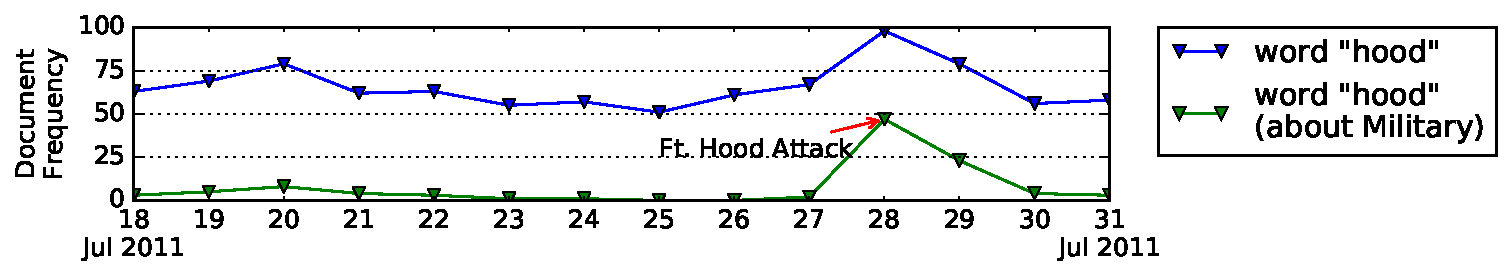
\includegraphics[width=1.0\columnwidth]{../img/hood.pdf}
        \caption{The comparison of the time series between the raw word \textit{hood} and the \textit{Military} related word \textit{hood}, computed on the \textit{Edinburgh twitter corpus}. The rise of document frequency on July 28th, 2011 is corresponding to the event mentioned in \url{https://en.wikipedia.org/wiki/Fort_Hood\#2011_attack_plot}.}
        \label{fig:hood}
\end{figure}
\end{frame}

%------------------------------
%page 7
\begin{frame}
\frametitle{The insights on the example}	

\end{frame}


%------------------------------
%page 8
\begin{frame}
\frametitle{Overview of our method}	

\begin{figure}[h]
		\setlength{\abovecaptionskip}{0.cm}
        \setlength{\belowcaptionskip}{0.cm}
        \centering
        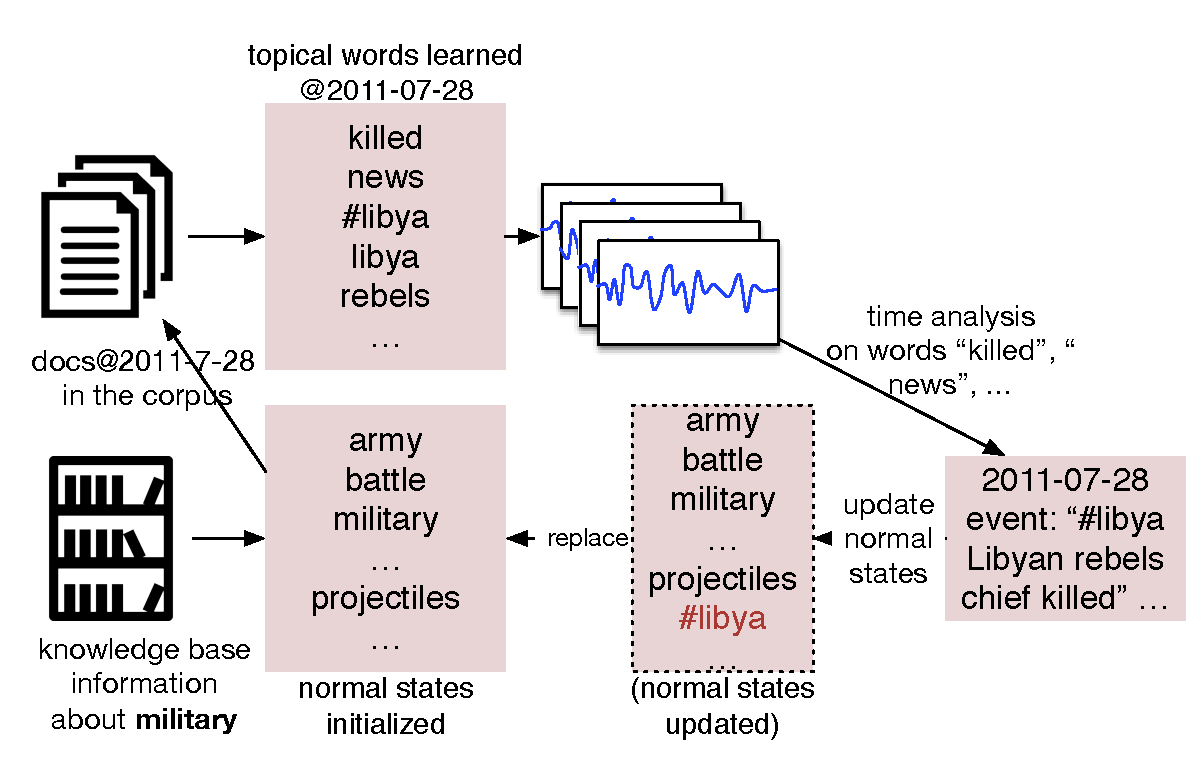
\includegraphics[width=0.5\columnwidth]{../img/NSDetectorExample.pdf}
        \caption{\textsc{TransDetector}'s processing flow, taking \textit{Military} related events in microblogs as an example.}
        \label{fig:hood}
\end{figure}


\end{frame}


%------------------------------
%page 9
\begin{frame}
\frametitle{\textsc{TransDetector}: Phrase 1}	
\begin{figure}[h]
		\setlength{\abovecaptionskip}{0.cm}
        \setlength{\belowcaptionskip}{0.cm}
        \centering
        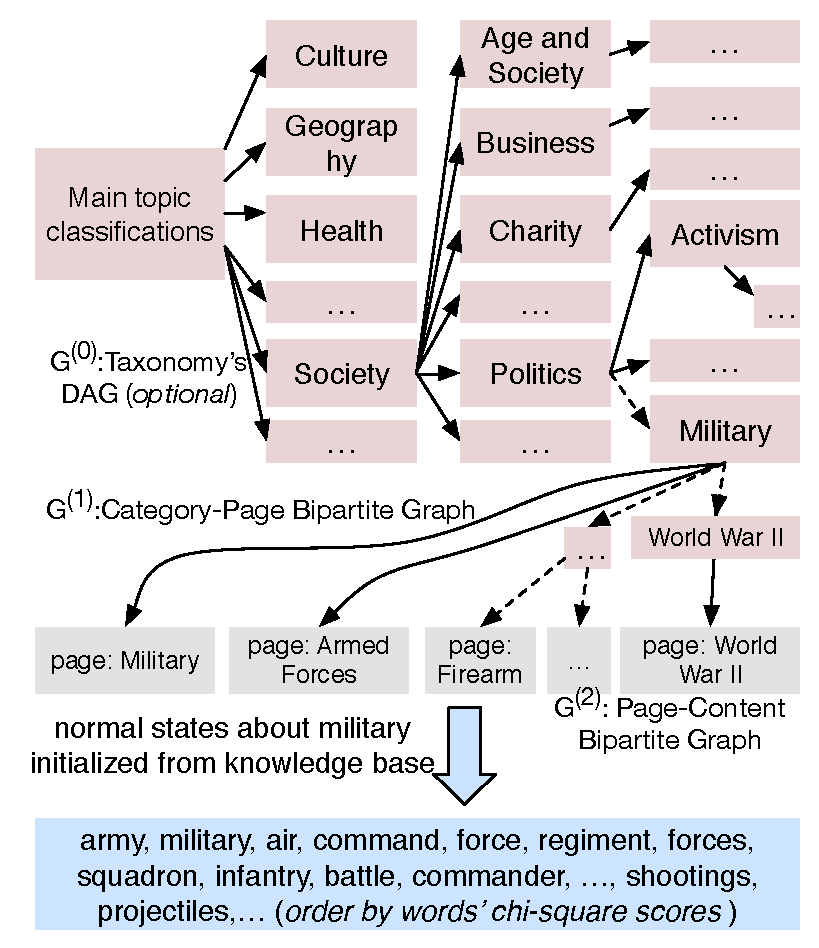
\includegraphics[width=0.5\columnwidth]{../img/initializationExample.pdf}
        \caption{Extracting Category-Level Topics in Knowledge Base via its three fold hierarchical structure, taking \textit{Military} as an example.}
        \label{fig:hood}
\end{figure}

\end{frame}

%------------------------------
%page 10
\begin{frame}
\frametitle{\textsc{TransDetector}: Phrase 2}	

\end{frame}

%------------------------------
%page 11
\begin{frame}
\frametitle{\textsc{TransDetector}: Phrase 3}	

\end{frame}


%------------------------------
%page 12
\begin{frame}
\frametitle{Experimental Results}	
\begin{figure}[h]
	\setlength{\abovecaptionskip}{0.cm}
	\setlength{\belowcaptionskip}{0.cm}
        \centering
        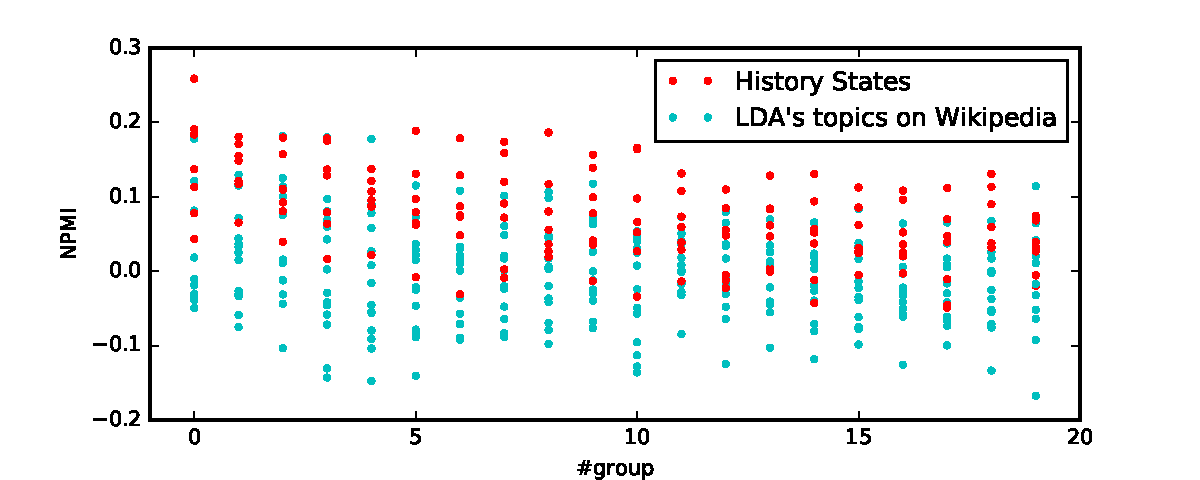
\includegraphics[width=1.0\columnwidth]{../img/NPMI.pdf}
        \caption{More topics are compared at the NPMI metrics between our method and LightLDA}
        \label{fig:NPMI}
\end{figure}
\end{frame}

\begin{frame}
\frametitle{some}

\begin{table}[h]
\setlength{\abovecaptionskip}{0.cm}%set the distance between caption and table to 0 cm.
\setlength{\belowcaptionskip}{0.cm}
\centering
\caption{The comparison on the topic coherence(NPMI) between our method and LightLDA, taking \textit{Aviation} as an example. (NPMI is computed on a group of ten words. \(\sim\) stands for the top five words.)}
\scalebox{0.45}{
\begin{tabular}{|c|l|l|c !{\vrule width 1pt} c|l|l|c|}
\hline
\multicolumn{4}{|c!{\vrule width 1pt}}{Category-Level Topics extracted from Wikipedia by \textsc{TransDetector}} & \multicolumn{4}{c|}{Topics Learned from Wikipedia by LightLDA}    \\ \hline
GID& \#words*  & words  & NPMI & GID& \#words*& words & NPMI \\ \hline
- & 1-5 & aircraft air airport flight airline &-& - & 1-5 & engine aircraft car air power &-\\ \hline
0 & 1-5, 6-10 & \(\sim\), airlines aviation flying pilot squadron &  0.113 & 0 & 1-5, 6-10 & \(\sim\), design flight model production speed & 0.112\\ \hline
1 & 1-5, 11-15 & \(\sim\), flights pilots raf airways fighter & 0.155 & 1 & 1-5, 11-15 &\(\sim\), system vehicle cars engines mm & 0.062\\ \hline
2 & 1-5, 16-20 & \(\sim\), boeing runway force crashed flew   & 0.092 & 2 & 1-5, 16-20 & \(\sim\), fuel vehicles designed models type & 0.072\\ \hline
3 & 1-5, 21-25 &\(\sim\), airfield landing passengers plane aerial & 0.179 & 3 & 1-5, 21-25 & \(\sim\), version front produced rear electric & 0.035\\ \hline
4 & 1-5, 26-30 &\(\sim\), bomber radar wing bombers crash & 0.137 & 4 & 1-5, 26-30 & \(\sim\), space control motor standard development & 0.085\\ \hline
5 & 1-5, 31-35 &\(\sim\), airbus airports operations jet helicopter & 0.189 & 5 & 1-5, 31-35 & \(\sim\), film range light using available & -0.002\\ \hline
6 & 1-5, 36-40 &\(\sim\), squadrons base flown havilland crew & 0.088 & 6 & 1-5, 36-40 & \(\sim\), wing powered wheel weight launch & 0.087\\ \hline
7 & 1-5, 41-45 & \(\sim\), combat luftwaffe aerodrome carrier fokker & 0.159 & 7 & 1-5, 41-45 & \(\sim\), developed low test ford cylinder & 0.007\\ \hline
8 & 1-5, 46-50 &\(\sim\), planes fly engine takeoff fleet & 0.186 & 8 & 1-5, 46-50 & \(\sim\), equipment side pilot hp aviation & 0.091\\ \hline
9 & 1-5, 51-55 &\(\sim\), fuselage helicopters aviator naval aero & 0.157 & 9 & 1-5, 51-55 & \(\sim\), systems us sold body drive & -0.051\\ \hline
10 & 1-5, 56-60 &\(\sim\), glider command training balloon faa & 0.166 & 10 & 1-5, 56-60 & \(\sim\), gear introduced class safety seat & 0.069\\ \hline
\(\cdots\) & \(\cdots\) &\(\cdots\) &\(\cdots\) & \(\cdots\) & \(\cdots\) &\(\cdots\) &\(\cdots\)\\ \hline
18 & 1-5, 96-100 &\(\sim\), scheduled carriers military curtiss biplane &0.131 & 18 & 1-5, 96-100 & \(\sim\), transmission special replaced limited different & 0.059\\ \hline
19 & 1-5, 101-105 &\(\sim\), accident engines iaf albatross rcaf &0.068 & 19 & 1-5, 101-105 & \(\sim\), features machine nuclear even unit & 0.011\\ \hline
\end{tabular}
}
\label{tbl:NPMIDetails}
\end{table}
	
\end{frame}

\begin{frame}
\frametitle{Experiment Settings}
	
\end{frame}



\begin{frame}
\frametitle{Experimental Results}	
\begin{table}
\setlength{\abovecaptionskip}{0.cm}%set the distance between caption and table to 0 cm.
\setlength{\belowcaptionskip}{0.cm}
\centering
\caption{Category-Level Topics extracted from knowledge base and the corresponding topics on microblog stream learned from CTrans-LDA. The words in \textbf{\textit{bold}} font are newly learned on the microblog stream by the transfer learning.}
\scalebox{0.55}{
\begin{tabular}{|cc|cc|cc|cc|cc|cc|}
\hline
\multicolumn{2}{|c|}{\textit{Aviation}} & \multicolumn{2}{c|}{\textit{Health}} & \multicolumn{2}{c|}{\textit{Middle East}} & \multicolumn{2}{c|}{\textit{Military}} & \multicolumn{2}{c|}{\textit{Mobile Phones}}\\
\begin{tabular}[c]{@{}c@{}}Knowledge\\ Base\end{tabular} & \begin{tabular}[c]{@{}c@{}}Microblog\\ Stream\end{tabular} & \begin{tabular}[c]{@{}c@{}}Knowledge\\ Base\end{tabular} & \begin{tabular}[c]{@{}c@{}}Microblog\\ Stream\end{tabular} & \begin{tabular}[c]{@{}c@{}}Knowledge\\ Base\end{tabular} & \begin{tabular}[c]{@{}c@{}}Microblog\\ Stream\end{tabular} & \begin{tabular}[c]{@{}c@{}}Knowledge\\ Base\end{tabular} & \begin{tabular}[c]{@{}c@{}}Microblog\\ Stream\end{tabular} & \begin{tabular}[c]{@{}c@{}}Knowledge\\ Base\end{tabular} & \begin{tabular}[c]{@{}c@{}}Microblog\\ Stream\end{tabular} \\ 
\hline
aircraft & air & health & weight & al & \textbf{\textit{\#syria}} & army & killed & android & iphone\\ 
air & plane & patients & loss & israel & \textbf{\textit{\#bahrain}} & military & news & mobile & apple \\ 
airport & flight & medical & diet & iran & people & air & \textbf{\textit{\#libya}} & nokia & android \\ 
flight & time & disease & health & arab & israel & command & libya & ios & app \\
airline & airlines & treatment & cancer & israeli & police & force & rebels & phone & ipad \\
airlines & news & hospital & lose & egypt & \textbf{\textit{\#libya}} & regiment & people & samsung & samsung \\
aviation & boat & patient & fat & egyptian & \#egypt & forces & police & game & mobile\\
flying & airport & clinical & tips & ibn & news & squadron & war & app & blackberry \\
pilot & force & symptoms & treatment & jerusalem & \textbf{\textit{\#israel}} & infantry & libyan & iphone & tablet \\
squadron & fly & cancer & body & syria & world & battle & attack & htc & apps\\
\hline
\end{tabular}
}
\label{tbl:historyStates}
\end{table}
\end{frame}

\begin{frame}
\frametitle{Experimental Results}	
\begin{table}[h]
\setlength{\abovecaptionskip}{0.cm}%set the distance between caption and table to 0 cm.
\setlength{\belowcaptionskip}{0.cm}
\centering
\caption{Overall Performance on Event Detection}

\scriptsize
\scalebox{0.75}{
\begin{threeparttable}  

\begin{tabular}{|c|c|c|c|c|c|c|}
    \hline
    Method & \begin{tabular}[c]{@{}c@{}}Number of\\Events to \\ be Evaluated \end{tabular} & \begin{tabular}[c]{@{}c@{}}Recall@ \\ Benchmark1\end{tabular}& \begin{tabular}[c]{@{}c@{}}Precision@ \\ Benchmark2\end{tabular} & \begin{tabular}[c]{@{}c@{}}Recall@ \\ Benchmark2\end{tabular} & \begin{tabular}[c]{@{}c@{}}F@ \\ Benchmark2\end{tabular} & \begin{tabular}[c]{@{}c@{}}DERate\tnote{a}\ \ (Duplicate\\ Event Rate)@\\ Benchmark2\end{tabular} \\ \hline
    LSH & 500 & 0.704 & 0.788 & 0.651 & 0.713 & 0.348 \\ \hline
    TimeUserLDA & 100 & 0.370 & 0.790 & 0.177 & 0.289 & 0.114 \\ \hline
    Twevent & 375 &  0.741 & 0.808 & 0.658 & 0.725 & 0.142 \\ \hline
    EDCoW & 349 & 0.556 & 0.748 & 0.511 & 0.607 & 0.226 \\ \hline
    BurstyBTM & 200 & 0.667 & 0.825 & 0.384 & 0.497 & \textbf{0.079} \\ \hline
    \textsc{TransDetector} & 457 & \textbf{0.889} & \textbf{0.912} & \textbf{0.876} & \textbf{0.894} & 0.170 \\ \hline
    \end{tabular}

\begin{tablenotes}  
\item[a] DERate = (the number of duplicate events) / (the total number of detected realistic events)
\end{tablenotes}  
\end{threeparttable}  
}
\label{tbl:overall}
\end{table}
\end{frame}

\begin{frame}
\frametitle{Experimental Results}	
\begin{figure}[h]
	\setlength{\abovecaptionskip}{0.cm}
	\setlength{\belowcaptionskip}{0.cm}
        \centering
        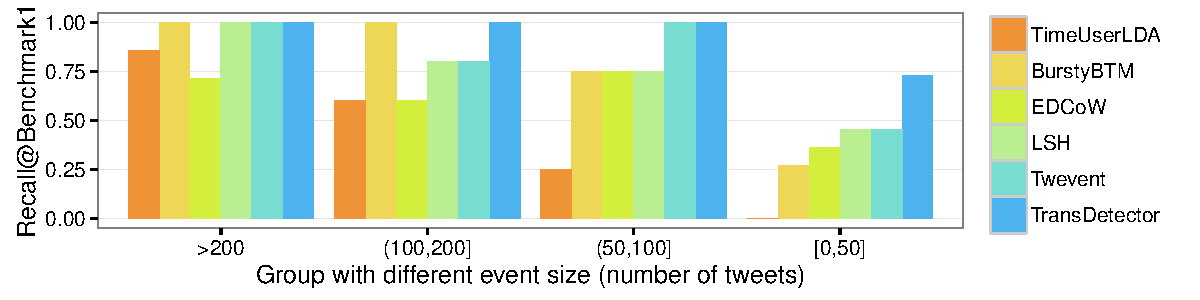
\includegraphics[width=1.0\columnwidth]{../img/barchartOnBenchmark1.pdf}
        \caption{The relation between the recall and the event size}
        \label{fig:Benchmark1}
\end{figure}
\end{frame}


\begin{frame}
\frametitle{Experimental Results}	
\begin{table}
\setlength{\abovecaptionskip}{0.cm}%set the distance between caption and table to 0 cm.
\setlength{\belowcaptionskip}{0.cm}
\centering
\caption{Events about \textit{military} detected by systems between 2011-07-22 and 2011-07-28}
\label{my-label}
\scalebox{0.6}{
\begin{threeparttable}  
\begin{tabular}{|c|l|l|c|c|c|c|c|c|c|}
\hline
\multirow{2}{*}{Date} & \multirow{2}{*}{Event key words} & \multirow{2}{*}{Representative event tweet} & \multirow{2}{*}{\begin{tabular}[c]{@{}l@{}}Number of \\ event tweet\end{tabular}} & \multicolumn{6}{c|}{Methods\tnote{a}} \\ \cline{5-10} 
 &  &  &  & L & TU & TW & E & B & TD \\ \hline
7/22/11 & \begin{tabular}[c]{@{}l@{}}Norway, Oslo,\\ attacks, bombing\end{tabular} & \begin{tabular}[c]{@{}l@{}}Terror Attacks Devastate Norway: A bomb\\ ripped through government offices in Oslo \\and a gunman... http://dlvr.it/cLbk8\end{tabular} & 557 & \checkmark & \checkmark & \checkmark & \checkmark & \checkmark & \checkmark \\ \hline
7/23/11 & Gunman, rink & \begin{tabular}[c]{@{}l@{}}Gunman Kills Self, 5 Others at Texas Roller\\ Rink http://dlvr.it/cLcTH\end{tabular} & 43 & - & - & \checkmark &  \checkmark & - & \checkmark \\ \hline
7/26/11 & \begin{tabular}[c]{@{}l@{}}Kandahar, mayor, \\ suicide, attack\end{tabular} & \begin{tabular}[c]{@{}l@{}}TELEGRAPH{]}: Kandahar mayor killed by\\ Afghan suicide bomber: The mayor of \\Kandahar, the biggest city in south \_\end{tabular} & 47 & \checkmark & - & \checkmark & \checkmark & - & \checkmark \\ \hline
7/28/11 & Ft., Hood, attack & \begin{tabular}[c]{@{}l@{}} Possible Ft. Hood Attack Thwarted\\ http://t.co/BSJ33hk\end{tabular} & 52 & - & - & - & - & - & \checkmark \\ \hline
7/28/11 & \begin{tabular}[c]{@{}l@{}}Libyan, rebel, \\ gunned\end{tabular} & \begin{tabular}[c]{@{}l@{}}Libyan rebel chief gunned down in Benghazi \\ http://sns.mx/prfvy1\end{tabular} & 44 & - & - & - & - & - & \checkmark \\ \hline
\end{tabular}

\begin{tablenotes}  
\item[a] L=LSH, TU=TimeUserLDA, TW=Twevent, E=EDCoW, B=BurstyBTM, TD=\textsc{TransDetector}.
\end{tablenotes}  
\end{threeparttable}  
}
\end{table}

\end{frame}


\begin{frame}
%\frametitle{A first slide}

\begin{center}
\Huge Thanks!
\end{center}

\begin{center}
\Huge Q\&A
\end{center}

%\begin{figure}[h]
%	\setlength{\abovecaptionskip}{0.cm}
%	\setlength{\belowcaptionskip}{0.cm}
%        \centering
%        
\includegraphics[width=0.3\columnwidth]{code.png}
%\end{figure}


\footnotetext{This slide and more data are available at \url{http://q-r.to/bajx8I}}

\end{frame}

%\end{comment}


\end{document}
